\documentclass{article}
\usepackage{times}
\usepackage{amsmath}
\usepackage{amsfonts}
\usepackage{fancyhdr}
\usepackage{amssymb}
\usepackage{tabularx}
\usepackage{listings}
\usepackage{graphicx}
\usepackage{enumerate}
\usepackage{cite}
\usepackage{amsthm}
\usepackage{color}
\usepackage{soul}
\usepackage[bookmarks,colorlinks=true,linkcolor=black,citecolor=black,urlcolor=blue]{hyperref}
\usepackage{authblk}
\usepackage{placeins}
\usepackage{longtable}

\definecolor{commentgreen}{RGB}{0,127,0}
\lstdefinelanguage[]{asn.1}%
  {keywords=%
    {DEFINITIONS,SEQUENCE,OCTET,INTEGER,BEGIN,END,OPTIONAL,STRING,IMPORTS,FROM,MODULE-IDENTITY,OBJECT IDENTIFIER},
    sensitive=true,
    comment=[l]{--}
  }[keywords]%
\lstset{
	commentstyle=\color{commentgreen}\textit,
	breaklines,
	numbers=left
}

\begin{document}

\title{IP-Controlled Low Voltage DC\\Power Distribution Unit\\ADVANCE DATASHEET}
\author{Andrew Zonenberg\\
	\texttt{azonenberg@drawersteak.com}}
\date{\today}
\maketitle

\fancyhead[L]{ADVANCE DATASHEET}
\fancyfoot[L]{$Revision$ / \today}
\pagestyle{fancy}

\setcounter{tocdepth}{2}
\tableofcontents

\pagebreak
\section{Introduction}

\subsection{Overview}
The PDU is an intelligent power distribution system for a large number (up to ten) of low voltage DC loads, such as 
encountered in a development board cluster for embedded prototyping. It is intended to consolidate many ``wall wart" 
power supplies into a single unit supplied by an external high-efficiency supply, saving outlet and workbench space 
while providing additional management and safety capabilities.

This is an advance specification of a system which is still under development. Some specifications are subject to 
change. Data marked as ``TBD" is dependent on characterization of prototype hardware.

\subsection{Feature summary}

\begin{itemize}
\item All functions of the device are accessible via SNMP using the on-board Gigabit Ethernet port.
\item Each output channel is individually switched to permit remote reset of a malfunctioning device under test (DUT).
\item Per-channel current metering allows real-time monitoring of current consumed by downstream loads, providing
instant feedback when optimizing DUT firmware for power.
\item Board-level reverse voltage protection guards against incorrect hookup of the upstream supply.
\item Input rail voltage is monitored internally and all outputs are disabled if the voltage deviates from nominal by 
more than a set threshold. A jumper on the board allows 5V or 12V mode to be selected and prevents damaging downstream 
devices if the PDU is accidentally connected to the wrong supply.
\item Two chassis temperature monitors allow thermal shutdown in the event of overload.
\item Programmable overcurrent shutdown for extremely rapid (several $\mu s$) shutdown of a shorting or malfunctioning
DUT. This protection responds significantly faster than a fuse and can be remotely reset once the fault condition has 
been cleared. Firmware allows flexible tailoring of overcurrent shutdown behavior including response time; a separate 
power-on threshold prevents false triggering from inrush currents.
\item Ten 3.3V  digital GPIO pins are provided for interfacing with external systems.
\item The entire system design (hardware and firmware) is released under a permissive open source license (3-clause
BSD). KiCAD design files and firmware source are available at \url{https://code.google.com/p/azonenberg-devboards/}
under the  subproject ``pdu-5v-20a". Modified firmware may be loaded onto the system via the provided JTAG header.
\end{itemize}

\pagebreak
\section{Physical Description}

\begin{figure}[h!]
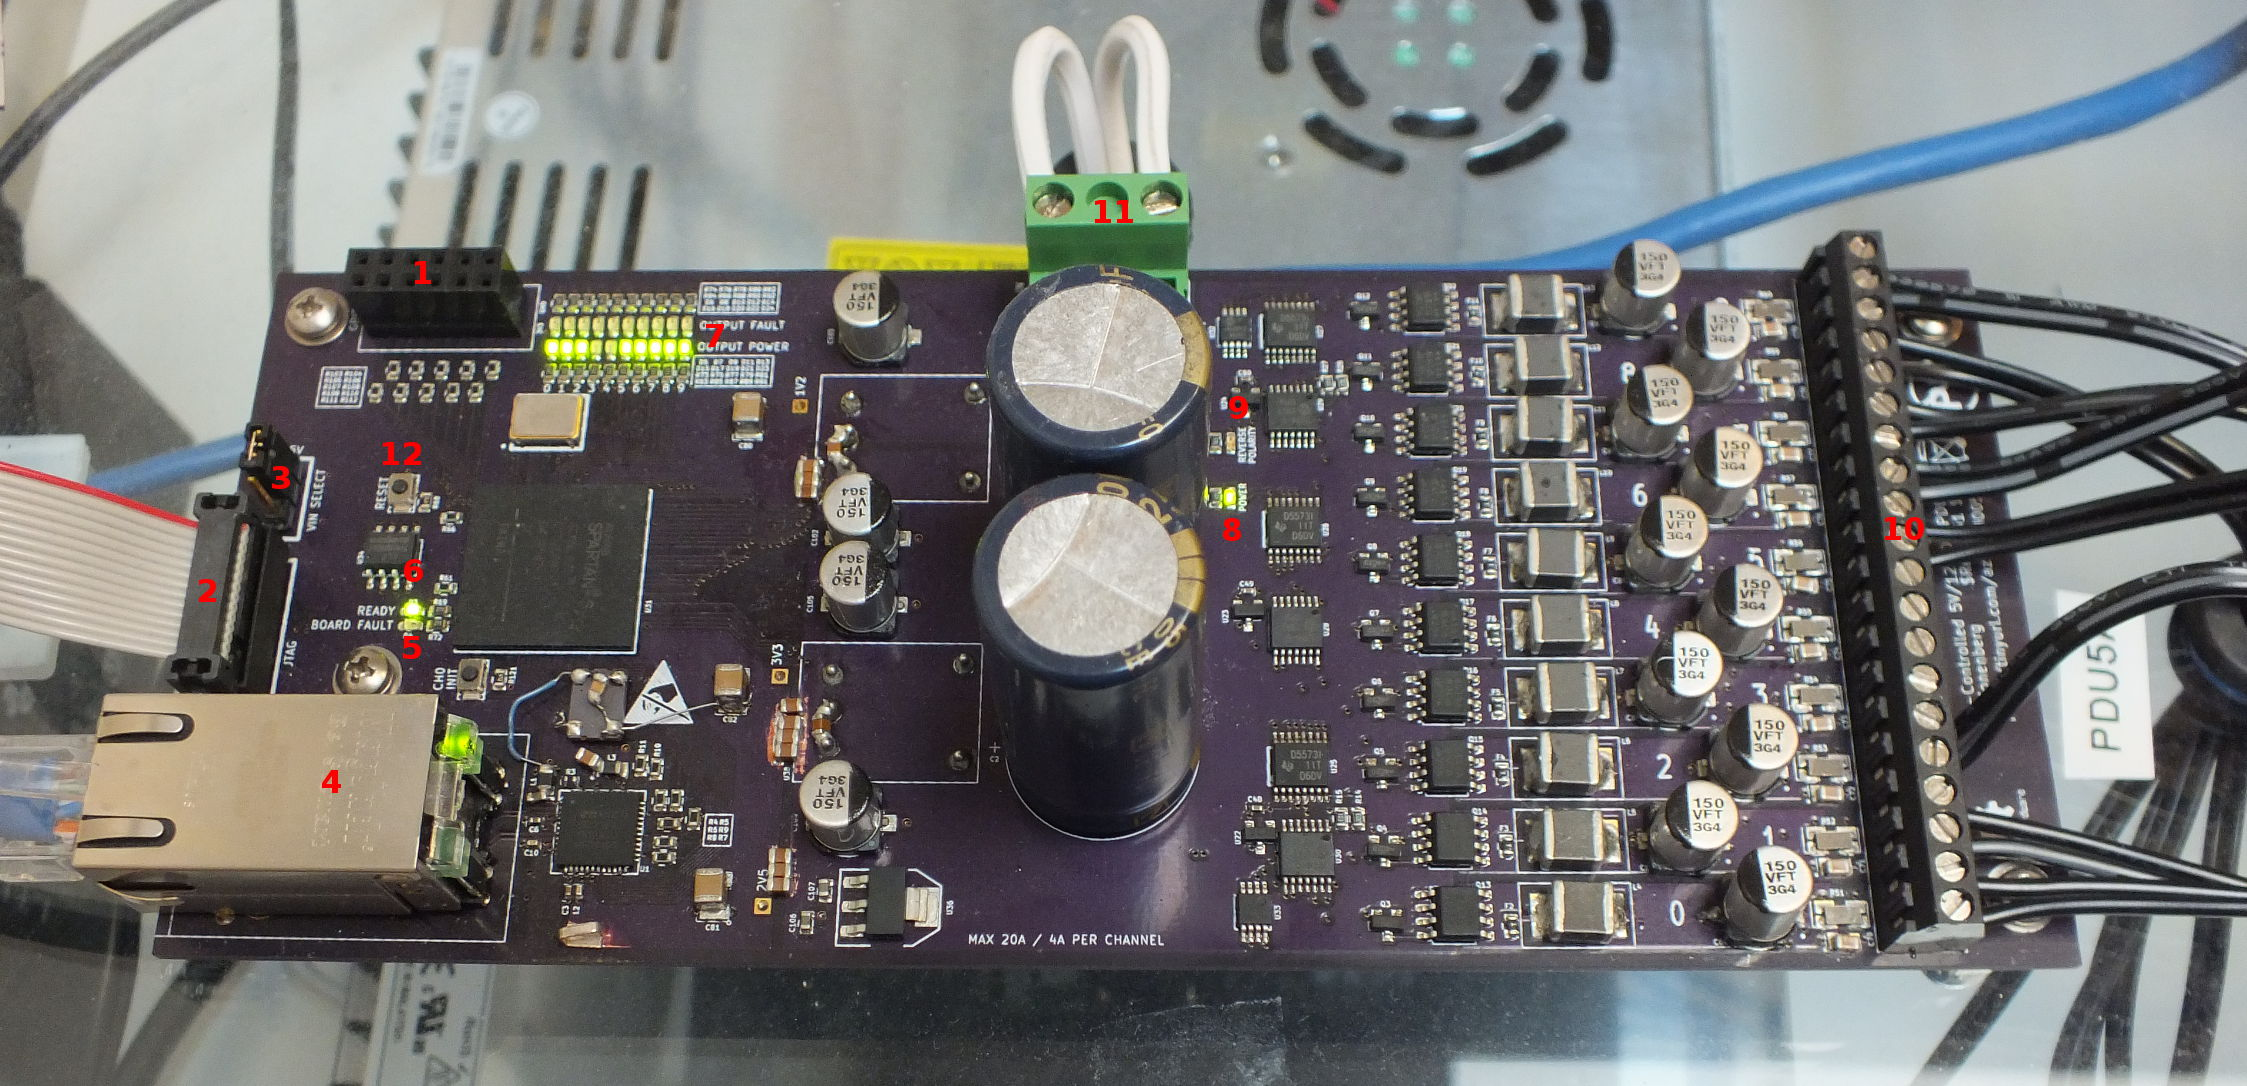
\includegraphics[scale=0.15]{board-overview.jpg}
\caption{PCB overview}
\label{board-overview}
\end{figure}
\FloatBarrier

TODO: Update image with nicer no-rework board once respin arrives.

The PDU is supplied as a printed circuit board with standoffs near each corner. There is no enclosure; the PDU is 
intended to be mounted inside a customer-supplied case as part of a larger system.

The board has the following connectors, controls, and indicators. For the remainder of this document, all references 
to ``left", ``right", ``top", and ``bottom" refer to the canonical board orientation in Fig. \ref{board-overview}.

TODO: Specify connector part numbers

\begin{longtable}{|l|p{4in}|}
\hline
{\bf Number} & {\bf Description}\\
\hline
1 & GPIO connector\\
\hline
2 & JTAG connector\\
\hline
3 & Voltage select jumper\\
\hline
4 & Ethernet RJ45 connector \\
\hline
5 & Board fault LED\\
\hline
6 & Ready LED\\
\hline
7 & Channel status LEDs\\
\hline
8 & Power LED\\
\hline
9 & Reverse voltage LED\\
\hline
10 & Power output terminals\\
\hline
11 & Power input terminals\\
\hline
12 & Reset button\\
\hline
\end{longtable}

\pagebreak
\section{Usage}

\subsection{Client System Requirements}

The PDU can communicate with any network management system implementing the industry standard Simple Network 
Management Protocol (SNMP). The MIB for the PDU is described in section \ref{sec:snmp}.

The official control GUI has only been tested on Debian 7 amd64 but should run on any recent Linux distribution. 
There are no plans to produce ports for other operating systems at this time however the software is open source and 
uses the cross-platform gtkmm UI toolkit so porting by end users is possible. Any patches or results of testing on 
other platforms will be appreciated.

No device drivers are required for clients. Any system capable of sending SNMP traffic over an Ethernet interface can 
communicate with the PDU.

\subsection{Firmware Updates}

The current firmware does not support remote firmware updates over the Ethernet interface. The provided JTAG header 
may be used with any standard Xilinx FPGA programming cable to load new firmware.

\subsection{Client Software}

TODO

\subsection{Status Indicators}

The board has several status indicator LEDs which provide visual feedback of system status. Most of this information 
may also be read remotely via the SNMP interface.

\begin{longtable}{|l|p{1.25in}|p{2.25in}|}
\hline
{\bf LED} & {\bf State} & {\bf Meaning}\\
\hline
Ethernet &
	Both off \newline
		Top green, bottom off \newline
		Other &
	No Ethernet link \newline
		Link up, normal operation \newline
		Ethernet link problem \\
\hline
Board fault &
	Off \newline
		Blinking red \newline
		Solid red &
	Normal operation \newline
		Thermal shutdown \newline
		Under/overvoltage shutdown \\
\hline
Ready & 
	Off \newline
		Green &
	FPGA still booting, or boot failure \newline
	Normal operation \\
\hline
Channel status & 
	Off \newline
		Green \newline
		Red &
	Output switched off \newline
		Output turned on \newline
		Overcurrent shutdown \\
\hline
Power &
	Off \newline
		Green &
	Board not powered, or input fuse blown \newline
		Normal operation \\
\hline
Reverse voltage &
	Off \newline
		Red &
	Normal operation \newline
		Board power connected backwards \\
\hline
\end{longtable}

\subsection{External connections}

\begin{itemize}

\item Connect an Ethernet cable from the RJ45 jack to the facility's LAN. 

\item Connect the green power-input terminals (11) to an external power supply capable of supplying 5V or 12V at a
minimum of 20 amps continuous duty. It is recommended that 14 gauge or larger stranded copper cabling be used. The input 
jack is labeled with a ``+" sign on the positive side (to the right, as seen in the photo).

\item Set the 5V / 12V jumper (3) to the appropriate position for the system operating voltage.

\item Connect the black power-output terminals (10) to the loads.

\item The GPIO header (1) is not used by the stock firmware and should be left unconnected. Custom firmware may use 
it for arbitrary digital I/O at LVCMOS33 levels.

\item The JTAG header (2) may be left disconnected during normal operation. A standard Xilinx JTAG cable may be connected 
for debug/test or firmware upgrade operations.

\end{itemize}

\subsection{Network configuration}

The board computes its MAC address by concatenating a locally administered prefix (02:), with a suffix chosen from the
last 24 bits of the FPGA's factory-programmed serial number (Device DNA). The resulting MAC address is printed on a
pressure-sensitive adhesive label on the underside of the board for easy identification.

The stock firmware does not support static IP addresses. As soon as the layer-2 link comes up the PDU will issue a 
DHCPDISCOVER request to the broadcast IP address. If a static IP is required, it should be assigned by the DHCP 
server based on the board's MAC address.

\subsection{Overcurrent protection}

All channels are protected against overcurrent. The limit may be set over the SNMP interface for each channel 
separately. When the limit is exceeded, the channel is switched off and the associated red LED is illuminated. The 
time from when the current first exceeds the limit until the output MOSFET is completely turned off is specified as 
$T_{ocs}$.

To clear the fault condition, simply switch the channel off and on again.

\begin{figure}[h!]
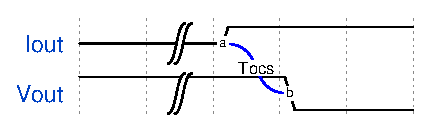
\includegraphics[scale=0.8]{Tocs.eps}
\caption{Overcurrent shutdown timing}
\label{tocs}
\end{figure}
\FloatBarrier

Each channel also has an inrush timer, which disables the soft overcurrent protection for a programmable number of 
milliseconds $T_{inrush}$ after power is switched on to prevent false triggering. Note that the passive fusing on 
output channels cannot be disabled. If the inrush limit is set too high it is possible to blow the fuse on the board 
before the soft protection trips. Such a fault will require a replacement fuse to be soldered on before the channel 
may be used again.

In the example below, the first power-on surge is shorter than $T_{inrush}$ so the output remains enabled until 
switched off. The second surge is longer than $T_{inrush}$ so overcurrent shutdown is triggered and the output turns 
off after $T_{ocs}$.

\begin{figure}[h!]
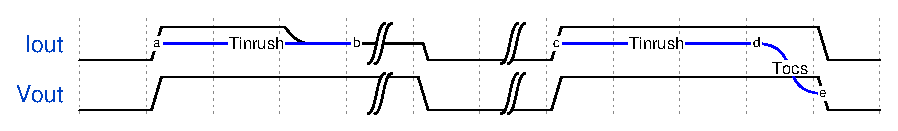
\includegraphics[scale=0.8]{Tinrush.eps}
\caption{Inrush timing}
\label{tinrush}
\end{figure}
\FloatBarrier

\subsection{Input reverse voltage protection}

The board is fully protected against reverse voltage up to the limits specified in section \ref{sec:dcchar}. 
Connecting input power backwards without exceeding these limits will result in the ``REVERSE VOLTAGE" LED 
illuminating and the board failing to boot, however no hardware damage will occur.

To clear the fault condition, remove input power and reconnect with the correct polarity.

\subsection{Board fault protection}

The board contains two thermal sensors which may be read at any time via the SNMP interface. If either of these 
sensors detect a reading outside of the recommended operating limits, firmware will shut down all outputs and blink 
the red ``BOARD FAULT" LED.

The board contains two voltage sensors which may be read at any time via the SNMP interface. If either of these 
sensors detect a reading outside of the recommended operating limits, firmware will shut down all outputs and 
steadily illuminate the red ``BOARD FAULT" LED.

A board fault condition may be cleared by pressing the soft reset button or power cycling the PDU.

\pagebreak
\section{Theory of operation}

\subsection{System overview}

The PDU requires an external (off board) 5V / 12V DC supply which should be capable of supplying at least 20A 
continuously. Power from the external connector is fed through a high-side PMOS based reverse voltage protection 
circuit to the primary power rail, which has two parallel 4700 $\mu F$ capacitors on it to smooth out load transients.

A tap on the primary power rail supplies power through two DC-DC converters and a linear regulator to the 3.3 / 2.5 / 
1.2V rails used by the FPGA, Ethernet PHY, and other control logic.

The primary power rail is then split off to the ten output stages (described below) which each supplies two screw 
terminals on the output connector. Outputs are not isolated; the input supply and all outputs share the same ground 
with high-side switching.

\begin{figure}[h!]
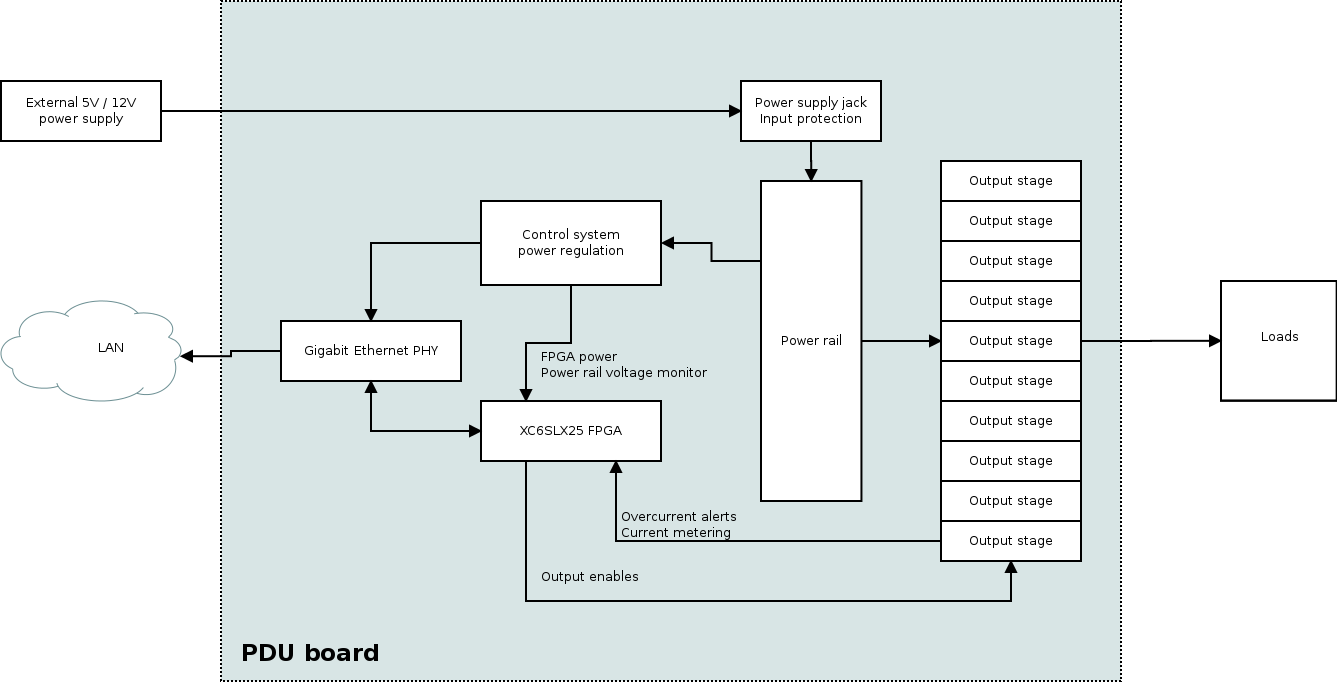
\includegraphics[scale=0.25]{system-block.png}
\caption{System block diagram}
\label{system-block}
\end{figure}
\FloatBarrier

\subsection{Output stage}

Each of the ten output channels is identically configured.

A 3.3V active-high output enable from the control logic is level-shifted to the power rail voltage by an N-channel
MOSFET, which then drives the gate of a high-side P-channel MOSFET. The switched power runs through a 5A fuse (as 
secondary protection in the event of an FPGA malfunction) and a ferrite chip to reduce coupling of EMI between 
downstream devices.The filtered power is then decoupled by a $150 \mu F$ electrolytic and $10 \mu F$ ceramic 
capacitor and fed through a $5 m\Omega$ shunt resistor to the output terminals.

\begin{figure}[h!]
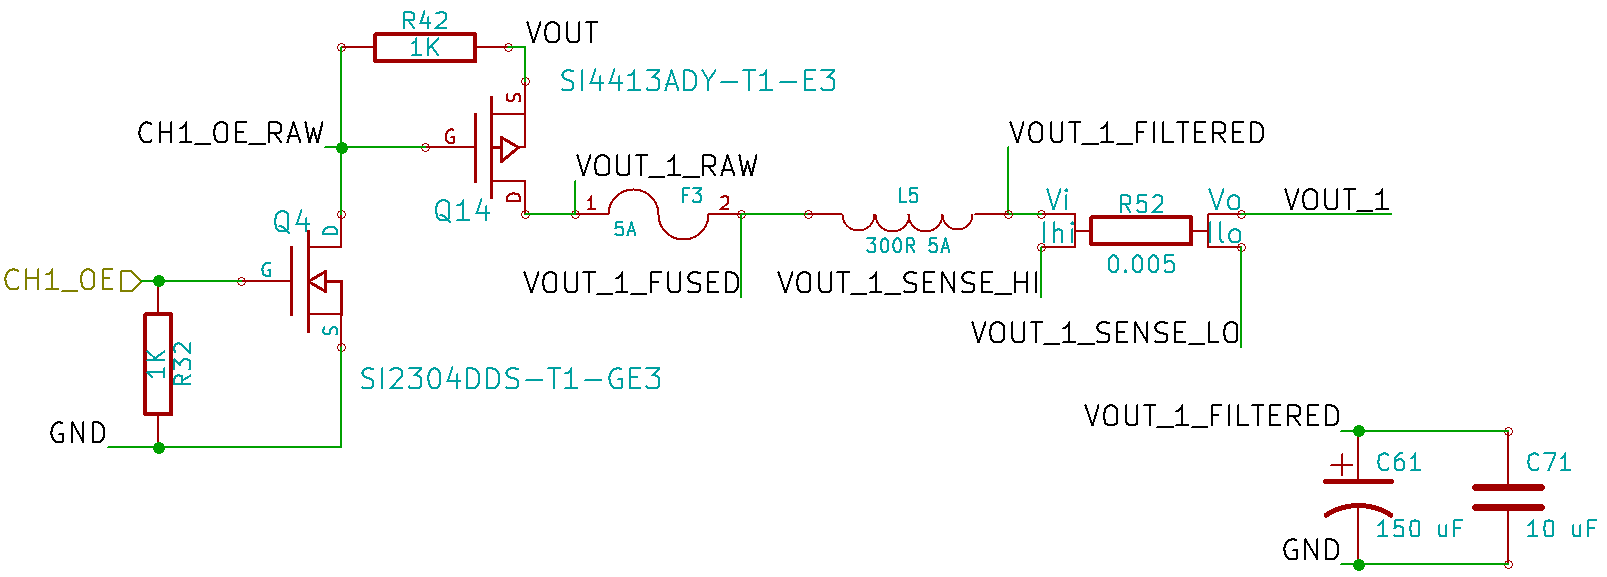
\includegraphics[scale=0.25]{output-stage-1.png}
\caption{Output stage circuit schematic}
\label{output-stage-1}
\end{figure}
\FloatBarrier

The shunt voltage is amplified 100x using by a Texas Instruments INA199A2 instrumentation amplifier to produce a 
voltage of 0.5V per A of output current and fed to a TLV3201 comparator. The resulting active-high overcurrent signal 
is sent to the FPGA, which will then shut down the output.

The comparator's reference voltage is supplied by a Texas Instruments DAC5573 8-bit DAC controlled over an I2C bus 
from the FPGA. One code value at the DAC corresponds to approximately 19.5 mA of current at the load. Note that the 
shunt resistor has a thermal coefficient of 50ppm and a tolerance of 1\%.

The stock firmware does not attempt to calibrate out ADC/DAC nonlinearity or shunt resistance variation, however the
FPGA has sufficient flash memory and block RAM to store per-board calibration values if required by custom firmware.

\begin{figure}[h!]
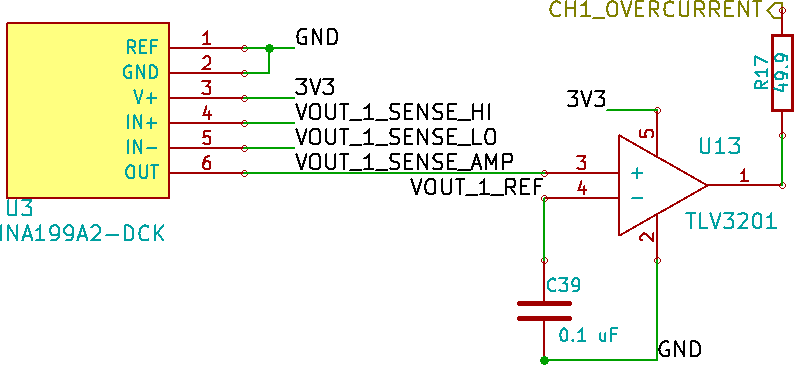
\includegraphics[scale=0.25]{output-stage-2.png}
\caption{Overcurrent detection circuit schematic}
\label{output-stage-2}
\end{figure}

Three Microchip MCP3204 12-bit 4-channel ADCs are connected to the amplified shunt voltage of each channel for metering
purposes, controlled by the FPGA over an SPI bus. A dedicated SPI bus is used for each of the three ADCs permitting
simultaneous sampling of of three values. The two remaining ADC channels are used to read the output rail voltage
(divided by six with 0.1\% tolerance $50K\Omega$ / $10K\Omega$ resistors to stay within the ADC's input range) at each
end of the power plane. 

One ADC code value corresponds to 1.22 mA at the load, or 2.44 mV of rail voltage in the first board revision. TODO: 
Update for next rev

\pagebreak
\section{SNMP interface}
\label{sec:snmp}

\subsection{Description}
TODO

\subsection{DRAWERSTEAK-MIB.my}
\lstinputlisting[language=asn.1]{/nfs/home/azonenberg/Documents/local/programming/achd-soc/trunk/src/PDUFirmware/DRAWERSTEAK-MIB.my}

\subsection{PDU-MIB.my}
\lstinputlisting[language=asn.1]{/nfs/home/azonenberg/Documents/local/programming/achd-soc/trunk/src/PDUFirmware/PDU-MIB.my}

\pagebreak
\section{Mechanical characteristics}

Four mounting holes (4-40 clearance size), one near each corner, are provided for mounting the board on standoffs to a 
workbench or enclosure.

All coordinates are relative to the upper left corner of the PCB.

\begin{figure}[h]
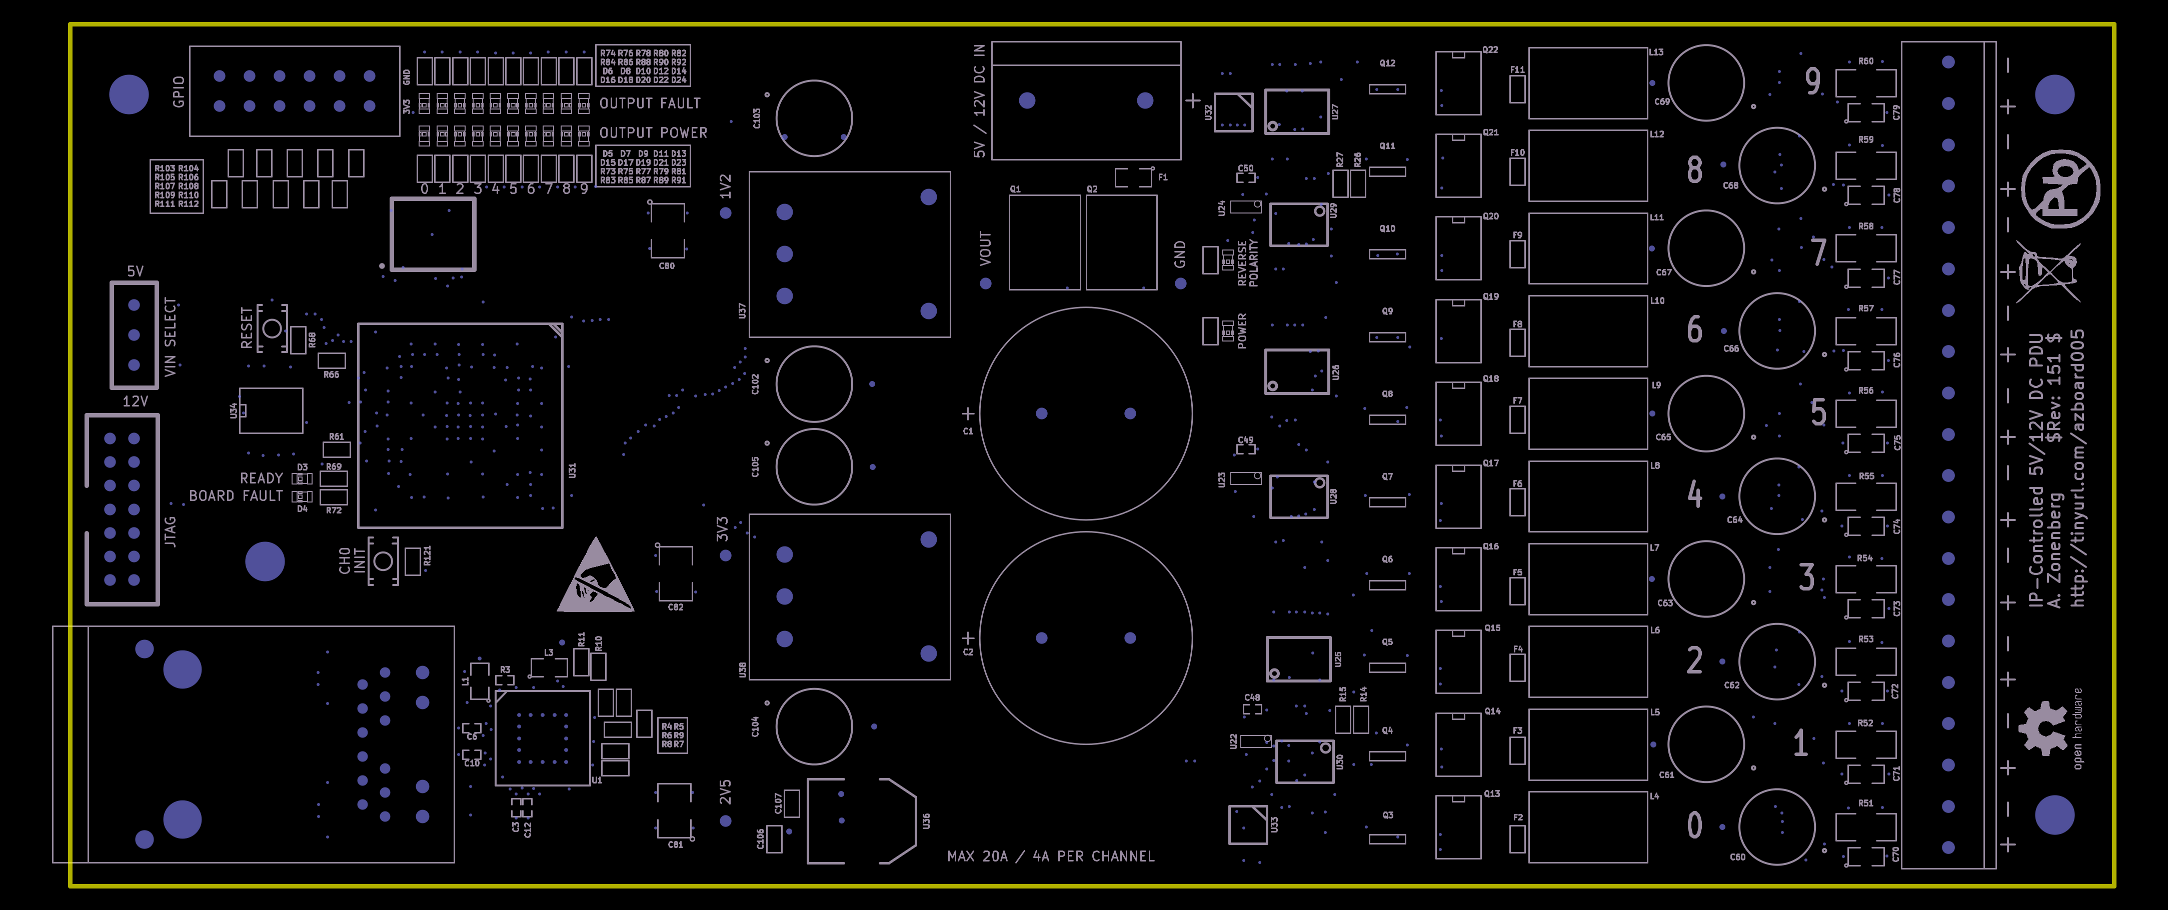
\includegraphics[scale=0.19]{silk-front-small.png}
\caption{PCB mechanical overview}
\label{silk-front}
\end{figure}

\begin{longtable}{|l|p{2in}|p{0.5in}|p{0.5in}|}
\hline
{\bf Symbol} & {\bf Description} & {\bf Typ} & {\bf Units}\\
\hline
$Len_{x}$ & Board size (horizontal axis) & 173 & mm\\
\hline
$Len_{y}$ & Board size (vertical axis) & 73 & mm\\
\hline
$DHole$ & Mounting hole diameter & 3.4 & mm\\
\hline
$Hole1_{x}$ & Mounting hole 1 X coordinate & 5.0 & mm\\
$Hole1_{y}$ & Mounting hole 1 Y coordinate & 6.0 & mm\\
\hline
$Hole2_{x}$ & Mounting hole 2 X coordinate & 16.5 & mm\\
$Hole2_{y}$ & Mounting hole 2 Y coordinate & 45.5 & mm\\
\hline
$Hole3_{x}$ & Mounting hole 3 X coordinate & 168.0 & mm\\
$Hole3_{y}$ & Mounting hole 3 Y coordinate & 6.0 & mm\\
\hline
$Hole4_{x}$ & Mounting hole 4 X coordinate & 168.0 & mm\\
$Hole4_{y}$ & Mounting hole 4 Y coordinate & 67.0 & mm\\
\hline
\end{longtable}

\pagebreak
\section{Operational characteristics}
\label{sec:dcchar}

\subsection{Absolute maximum ratings}

Stresses above these limits may cause permanent damage to the board. This is a stress rating only and functional
operation at these conditions, or any conditions outside of the specified operational characteristics, is not implied.

\begin{longtable}{|l|p{2in}|p{0.5in}|p{0.65in}|p{0.5in}|}
\hline
{\bf Symbol} & {\bf Description} & {\bf Min} & {\bf Max} & {\bf Units}\\
\hline
$V_{in}$ & Supply voltage & -20 & 15.6 & V\\
\hline
$V_{outrev}$ & DC voltage applied to power output & -0.25 & $V_{in} + 0.5$ & V\\
\hline
$I_{in}$ & Input current (sum of control logic and all active outputs) & & 25 \footnote{Input fuse rating} & A\\
\hline
$I_{out}$ & Output current per channel & & 5 \footnote{Output fuse rating} & A\\
\hline
$T_{pcb}$ & Board temperature & 0 & 65 & $^{\circ}$C\\
\hline
\end{longtable}

\subsection{Recommended operating conditions}

The board is specified to operate normally within these limits. Exceeding these limits may result in firmware 
triggering a panic shutdown to protect downstream devices.

Since the board may operate in either 5V mode or 12V mode some voltage measurements are referenced to $V_{nom}$, the 
nominal supply voltage.

\begin{longtable}{|l|p{2in}|p{0.75in}|p{0.5in}|p{0.75in}|p{0.4in}|}
\hline
{\bf Symbol} & {\bf Description} & {\bf Min} & {\bf Typ} & {\bf Max} & {\bf Units}\\
\hline
$V_{nom}$ &
	(5V mode) Nominal supply voltage
	\newline (12V mode) &
	&
	5.00 \newline 12.00 &
	&
	V\\
\hline
$V_{in}$ &
	Supply voltage \footnote{Firmware shutdown limits} &
	$V_{nom} - 0.25$ &
	$V_{nom}$ &
	$V_{nom} + 0.25$ &
	V\\
\hline
$I_{in}$ & Input current & & & 20 & A\\
\hline
$I_{out}$ & Output current per channel & & & 4 & A\\
\hline
$T_{pcb}$ & Board temperature \footnote{Firmware shutdown limits} & 5 & & 60 & $^{\circ}$C\\
\hline
\end{longtable}

\subsection{DC performance characteristics}

Typical values are measured by characterization and not guaranteed.

\begin{longtable}{|l|p{2.5in}|p{0.5in}|p{0.5in}|p{0.5in}|p{0.5in}|}
\hline
{\bf Symbol} & {\bf Description} & {\bf Min} & {\bf Typ} & {\bf Max} & {\bf Units}\\
\hline
$R_{s(on)}$ & DC resistance from input to enabled output & & 50 & & $m\Omega$\\
\hline
$R_{s(off)}$ & DC resistance from input to disabled output & 0.5 & & & $M\Omega$\\
\hline
$I_{pdu}$ & (5V mode) PDU logic supply current \newline (12V mode) & & 0.3 \newline TBD &  & A\\
\hline
\end{longtable}

\section{AC / timing characteristics}

\subsection{Timing data}

\begin{longtable}{|l|p{2in}|p{0.5in}|p{0.65in}|p{0.65in}|p{0.5in}|}
\hline
{\bf Symbol} & {\bf Description} & {\bf Min} & {\bf Typ} & {\bf Max} & {\bf Units}\\
\hline
$T_{pu}$ & Power-up time & & TBD & & sec\\
\hline
$T_{ocs}$ & Overcurrent shutdown time & & 15 & & $\mu s$\\
\hline
\end{longtable}

\pagebreak
\section{Errata}

\subsection{Ethernet speeds}

The current firmware version supports full duplex 1000 Mbps mode only. 10/100 mode and half duplex are not 
supported.

\pagebreak
\section{Legal}

\subsection{Notes}

Advance specifications are subject to change.

This board is NOT currently FCC, UL, or CE certified. End users are responsible for obtaining any required 
certifications needed.

\subsection{License and disclaimers}
                                                                                                                   
Copyright (c) 2012-2013 Andrew D. Zonenberg. All rights reserved.

Redistribution and use in source, bitstream, or layout form, with or without modification, is permitted
provided that the following conditions are met:

\begin{itemize}
\item Redistributions of source code must retain the above copyright notice, this list of conditions, and the following
disclaimer.

\item Redistributions in bitstream or layout form must reproduce the above copyright notice, this list of conditions and
the following disclaimer in the documentation and/or other materials provided with the distribution.

\item Neither the name of the author nor the names of any contributors may be used to endorse or promote products
derived from this hardware or software without specific prior written permission.

\item THIS SOFTWARE AND HARDWARE DESIGN IS PROVIDED BY THE AUTHOR "AS IS" AND ANY EXPRESS OR IMPLIED WARRANTIES, 
INCLUDING, BUT NOT LIMITED TO, THE IMPLIED WARRANTIES OF MERCHANTABILITY AND FITNESS FOR A PARTICULAR PURPOSE ARE 
DISCLAIMED. IN NO EVENT SHALL THE AUTHOR BE HELD LIABLE FOR ANY DIRECT, INDIRECT, INCIDENTAL, SPECIAL, EXEMPLARY, OR 
CONSEQUENTIAL DAMAGES (INCLUDING, BUT NOT LIMITED TO, PROCUREMENT OF SUBSTITUTE GOODS OR SERVICES; LOSS OF USE, 
DATA, OR PROFITS; OR BUSINESS INTERRUPTION) HOWEVER CAUSED AND ON ANY THEORY OF LIABILITY, WHETHER IN CONTRACT, 
STRICT LIABILITY, OR TORT (INCLUDING NEGLIGENCE OR OTHERWISE) ARISING IN ANY WAY OUT OF THE USE OF THIS SOFTWARE OR 
HARDWARE, EVEN IF ADVISED OF THE POSSIBILITY OF SUCH DAMAGE.

\end{itemize}

\end{document}


